\chapter{Gaussian processes}

\section{Parametric and nonparametric regression}
Consider the standard regression problem: given $\mathcal{D} = \{(x_i,y_i)\}_{i=1}^N$, with $x_i \in \mathcal{X}$ and $y_i \in \mathbb{R}$, one wants, for a $x_* \in \mathcal{X}$, find $p(y_*|x_*)$. If we assume a model $M$ for $y|x$, for all $x \in \mathcal{X}$, parameterized by $\theta$, then by the Bayesian view one should marginalize over $\theta$ resulting in 
\begin{equation}
 p(y_*|x_*,M,\mathcal{D}) = \int_{\Theta} p(y_*|x_*,\theta,M,\mathcal{D}) p(\theta|\mathcal{D}) d\theta,
\end{equation}
reducing the problem to one of posterior inference in $\theta$, discussed in the previous chapter (equation \eqref{marginalizationpred}).

Since the model $M$ is parameterized, in a sense the model will be always limited, since there cannot be a mapping from finite parameters to all distributions. Nonparametric models by contrast are models that cannot be parameterized by a finite set of parameters, and Bayesian nonparametric regression is when a nonparametric model is used in the Bayesian setting \cite{Ghahramani_2013,Hjort_2010}. 

\section{Gaussian process regression}
Bayesian nonparametric regression seems to be an impossible task, since it requires working with distributions in infinite-dimensional spaces. However, Gaussian process regression \cite{Rasmussen06} does this, by choosing a suitable model, given by a Gaussian process
\begin{Definition}
	A \textit{Gaussian process} (GP) is a distribution over the space of functions from $\mathcal{X}$ to $\mathbb{R}$ such that, for each $\mathbf{x} = (x_1,...,x_N) \in \mathcal{X}^N$, $\mathbf{f} := (f(x_1),...,f(x_N))$ follows a multivariate normal distribution \cite{Rasmussen06}. 
\end{Definition}

A GP is completely specified by a \textit{mean function}
\begin{displaymath}
m : \mathcal{X} \to \mathbb{R}
\end{displaymath}
and a \textit{covariance function} 
\begin{displaymath}
k : \mathcal{X} \times \mathcal{X} \to \mathbb{R},
\end{displaymath}
in such a way that, for $\mathbf{x} = (x_1,\ldots,x_N)$, letting
\begin{equation}
\mathbf{m}(\mathbf{x}) := (m(x_1),...,m(x_N))^T \quad K(\mathbf{x},\mathbf{x}') = \bigg(k(x_i,x_j')\bigg)_{i,j},
\end{equation}
then $f(\mathbf{x}) \sim \mathcal{N}(\mathbf{m}(\mathbf{x}),K(\x,\x))$. 

Notice that this requires the function $k$ to be a \textit{positive-semidefinite} (PSD) function, that is, for any $N \in \mathbb{N}$, for any $\mathbf{x} = (x_1,...,x_N) \in \mathcal{X}^N$, the matrix $K(\mathbf{x},\mathbf{x})$ defined by $(K(\mathbf{x},\mathbf{x}))_{i,j} = k(x_i,x_j)$ is PSD. Conversely, any pair $(m,k)$, with $k$ PSD defines a GP \cite{Dudley_2002}, thus ensuring a correspondence between GPs and $(m,k)$ pairs as above. In the context of GPs, $k$ is also called an \textit{kernel}. \footnote{PSD functions have the property that, for $x,x' \in \mathcal{X}$, $k(x,x') = \langle \Phi(x), \Phi(x') \rangle_{\mathcal{H}}$, where $\Phi : \mathcal{X} \to \mathcal{H}$ is a map from $\mathcal{X}$ to a Hilbert space $\mathcal{H}$ \cite{Shawe_Taylor_2004}. In this context, $k$ is called a \textit{kernel function}, and machine learning techniques that uses them are called kernel methods \cite{Shawe_Taylor_2004}. Hence, in the context of GPs, the terms \textit{kernel function} and {covariance function} are used interchangeably.}

A \textit{Gaussian process regression} is done, with $\mathcal{D} = \{(x_i,y_i)\}_{i=1}^N$, by using the model $M$ that says, for each $x$, $p(y|x,M) = p(y|f(x),M)$, with the prior for $f$ being distributed as $GP(m,k)$. To see that this prior is attractive, assume for now $y = f(x)$. By letting $\mathbf{x} = (x_1,\ldots,x_N)$ \footnote{Usually, $x_i \in \mathbb{R}^D$, and $\mathbf{x}$ is written as a matrix whose $i$-th row is $x_i$. In this case, we may use $\mathbf{X}$ to denote this matrix instead, and reserve $\mathbf{x}$ to denote each point in $\mathbb{R}^D$. We will however use a more general notation.} and $\mathbf{y} = (y_1,\ldots,y_N)^T$, and assuming $K(\mathbf{x},\mathbf{x})$ to be non-singular, one can find the posterior distribution for $y_*|x_*,\mathcal{D},M$ without resorting to Bayes' rule, which is important since, in infinite-dimensional spaces, Bayes' rule is more involved, and may not result in a computable expression by itself \cite{Kanagawa_2018}. \footnote{For a derivation of Bayes' rule for infinite-dimensional spaces (which involves measure theory), see \cite{Stuart_2010}, Section 6.6.}

Too see why is this, notice that, by the definition of a GP, for any other $\mathbf{x}^\star \in \mathcal{X}^M$, 
\begin{equation} \label{jointGP}
\left[ \begin{array}{c} 
f(\mathbf{x}) \\
f(\mathbf{x}^*) \end{array} \right] \sim \mathcal{N} 
\left( \left[ \begin{array}{c}
\mathbf{m}(\mathbf{x}) \\
\mathbf{m}(\mathbf{x}^*) \end{array} \right] , 
\left[ \begin{array}{c c} 
K(\mathbf{x},\mathbf{x}) & K(\mathbf{x},\mathbf{x}^*) \\
K(\mathbf{x}^*,\mathbf{x}) & K(\mathbf{x}^*,\mathbf{x}^*) \end{array} \right]
\right).
\end{equation}
Hence, by conditioning on $f(\mathbf{x})$, by Appendix \ref{appendixconditional}:
\begin{equation}\label{meancovGPRpure}
\begin{split}
& f(\mathbf{x}^*) | \mathbf{x}^\star, \mathcal{D}, M = \mathbf{f}^*|\mathbf{f},M \sim \mathcal{N}(\mu^\star,\Sigma^*) \\
& \mu^\star = \mathbf{m}(\mathbf{x}^\star) + K(\mathbf{x}^\star,\mathbf{x}) K(\mathbf{x},\mathbf{x})^{-1} (f(\mathbf{x}) - m(\mathbf{x})) \\
& \Sigma^\star = K(\mathbf{x}^\star,\mathbf{x}^\star) - K(\mathbf{x}^\star,\mathbf{x}) K(\mathbf{x},\mathbf{x})^{-1} K(\mathbf{x},\mathbf{x}^\star).
\end{split}
\end{equation}
Since $\x^*$ was chosen arbitrarily, this implies that $f|\mathcal{D},M$ itself follows a GP, with mean function and covariance functions given by:
\begin{equation}\label{GPRasGP}
\begin{split}
& m_{\mathcal{D}}(x) = \mu^*(x) = m(x) + K(x,\mathbf{x}) K(\mathbf{x},\mathbf{x})^{-1} (f(\mathbf{x}) - m(x)) \\
& k_{\mathcal{D}}(x,x') = k(x,x') - K(x,\mathbf{x}) K(\mathbf{x},\mathbf{x})^{-1} K(\mathbf{x},x').
\end{split}
\end{equation}
Since $y_* = f(x_*)$ and $\mathbf{y} = f(\mathbf{x}^*)$, $y_*|x_*,\mathcal{D},M \sim \mathcal{N}(m_\mathcal{D}(x_*),k_\mathcal{D}(x_*,x_*))$. An illustration of GP regression is shown if Figure \ref{gprfig}.

\begin{figure}
	\centering
	\subfloat[GP prior]{\label{gprex1a}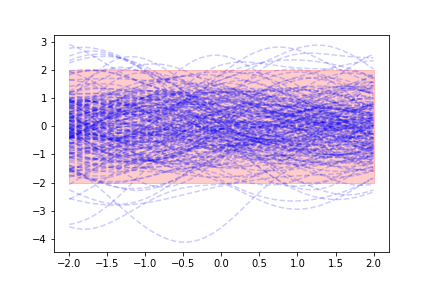
\includegraphics[width=0.45\textwidth]
		{figs/gprex1a.png}}
	\subfloat[GP posterior]{\label{gprex1b}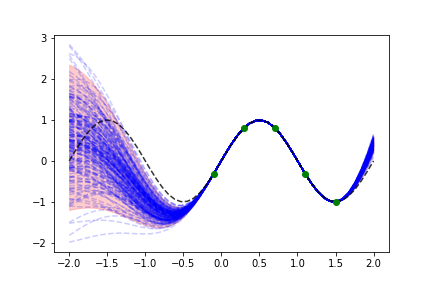
\includegraphics[width=0.45\textwidth]
		{figs/gprex1b.png}}
	
	\caption[Gaussian process regression of $f(x) = \sin(\pi x)$]{\label{gprfig}Gaussian process regression of $f(x) = \sin(\pi x)$. In (a), it is shown the prior space distribution, with samples path in blue and confidence interval in red. In (b), the posterior space distribution, after 4 measurements (in green) of $f(x)$ (black). Generating code can be found in \url{https://github.com/DFNaiff/Dissertation/blob/master/illustrations_dissertation/gp_prior_posterior}.}
\end{figure}


\subsection{Gaussian noise}
This equation can be generalized by assuming $p(y|x,M) = \mathcal{N}(y|f(x),\sigma^2_n)$. Then, letting $\epsilon \sim \mathcal{N}(0,\sigma^2_n)$, $\mathbf{y} = f(\mathbf{x})$, $\mathbf{y}^* = f(\mathbf{x}^*)$ and
\begin{equation} \label{jointGPnoise}
\left[ \begin{array}{c} 
\mathbf{y} \\
\mathbf{y}^* \end{array} \right] \sim \mathcal{N} 
\left( \left[ \begin{array}{c}
\mathbf{m}(\mathbf{x}) \\
\mathbf{m}(\mathbf{x}^*) \end{array} \right] , 
\left[ \begin{array}{c c} 
K(\mathbf{x},\mathbf{x}) + \sigma_n^2 I & K(\mathbf{x},\mathbf{x}^*) \\
K(\mathbf{x}^*,\mathbf{x}) & K(\mathbf{x}^*,\mathbf{x}^*) + \sigma^2_n I \end{array} \right]
\right).
\end{equation}
Conditioning $\mathbf{y}^*$ on $\mathbf{y}$ and, letting $K_\sigma(\mathbf{x},\mathbf{x}) := K(\mathbf{x},\mathbf{x}) + \sigma_n I$, we have
\begin{equation}\label{meancovGPR}
\begin{split}
& \mathbf{y}^* | \mathbf{x}^\star, \mathcal{D}, M = \mathbf{y}^*|\mathbf{y},M \sim \mathcal{N}(\mu^\star,\Sigma^*) \\
& \mu^\star = \mathbf{m}(\mathbf{x}^\star) + K(\mathbf{x}^\star,\mathbf{x}) K_\sigma(\mathbf{x},\mathbf{x}){-1} (\mathbf{y} - m(\mathbf{x})) \\
& \Sigma^\star = K(\mathbf{x}^\star,\mathbf{x}^\star) - K(\mathbf{x}^\star,\mathbf{x}) K_\sigma(\mathbf{x},\mathbf{x})^{-1} K(\mathbf{x}^\star,\mathbf{x}) + \sigma_n I.
\end{split}
\end{equation}
Notice \eqref{meancovGPR} reduces to \eqref{meancovGPRpure} when $\sigma^2_n = 0$. 
\subsection{General noise}
In the general case where $p(y|x,M)$ = $p(y|f(x))$, there is not a closed form solution and one must resort to explicit marginalization and Bayes' rule:
\begin{equation}\label{generalnoise}
\begin{split}
 & p(y_*|x_*,\mathcal{D}) = \\  & = 
  \int p(y_*|f(x_*)) p(f(x_*)|x_*,\mathbf{x},\mathbf{y}) df(x_*)\\ & = 
  \int p(y_*|f(x_*)) \int p(f(x_*)|x_*,f(\mathbf{x}), \mathbf{x}) p(f(\mathbf{x}) | \mathbf{x},\mathbf{y}) df(\mathbf{x}) df(x_*) \\ & \propto
  \int p(y_*|f(x_*)) \int p(f(x_*)|x_*,f(\mathbf{x}), \mathbf{x}) p(\mathbf{y}|f(\mathbf{x})) p(f(\mathbf{x})|\mathbf{x}) df(\mathbf{x})df(x_*).
 \end{split}
\end{equation}
Since $p(f(\mathbf{x})|\x) = \mathcal{N}(f(\mathbf{x})|m(\mathbf{x}),K(\mathbf{x},\mathbf{x}))$ and $p(f(x_*)|x_*,f(\mathbf{x}), \mathbf{x})$ is given by \eqref{meancovGPRpure}, these two terms may be joined together by \eqref{productgaussians}. However, this still leaves a double integral, that must be treated by approximate inference methods.

\subsection{Mean function}
Usually, the mean function $m$ is set to zero, letting the covariance function determine the whole structure of the regression. This is a reasonable assumption since, for any $f \sim GP(m,k)$, due to the sum of a Gaussian distribution and a constant being itself Gaussian with the constant added to its mean, we have $f-m \sim GP(0,k)$. Thus, fixed the model $(m,k)$, one can then do the GP regression on $f-m$ and then later add $m$. This is particularly useful if it is assumed that $f$ is modeled by some function $m$ that is known to be an incomplete model, thus complementing the regression by modeling this incompleteness by a zero mean GP.

\section{Covariance functions}

As said in the previous section, covariance functions $k$ must be PSD. This raises the question on which kind of functions are PSD, thus able to define a GP. A few functions can be easily shown to be PSD directly by their definitions, such as:
\begin{itemize}
	\item The constant function $k(x,x') = c \geq 0$, since the matrix $K_{i,j} = c$ is PSD, for all $c \geq 0$
	\item $k(x,x') = \mathbb{I}_{x = x'}$, since the corresponding matrix $K$ is the identity matrix
	\item If $\mathcal{X} = \{x_1,...,x_N\}$  is a finite set of size $N$, and $k$ is such that, for $\mathbf{x} = (x_1,...,x_N)$, 
	$K(\mathbf{x},\mathbf{x})$ is PSD, then $k$ is PSD, since for any other subset of $\mathcal{X}$, the corresponding kernel matrix will be a subset of $K$, thus also PSD \cite{hogben14}.
	\item If we have an explicit feature map $\Phi : \mathcal{X} \to \mathbb{R}^N$, then $k(x,x') = \langle \Phi(x),\Phi(x') \rangle$ is PSD \cite{Shawe_Taylor_2004}. For instance, if $\mathcal{X} = \mathbb{R}$ and $\Phi(x) = (x,x^2,\ldots,x^N)$, then $k(x,x') = \sum_{i=1}^N (x x')^i$ is PSD.
\end{itemize}
However, for many covariance functions, direct proof of being PSD is infeasible. However, there are some covariance functions that can be shown to be PSD in a indirect way, as shown below.
\subsubsection{Stationary covariance functions}
\begin{Definition}
	Let $\mathcal{X} = \mathbb{R}^d$. An covariance function is \textit{stationary} if $k(x,x') = k(x - x')$ , 
	for $k : \mathbb{R}^d \to \mathbb{R}$ \footnote{Here we overload the notation, letting the reader infer whether $k$ refers to a covariance function or an autocavariance function by the number of its arguments.}. Conversely, $k$ is a \textit{autocovariance function} if $k(x,x') = k(x - x')$ is a covariance function.
\end{Definition}
For this class of functions, we can reduce the analysis of $k$ to that of $k$. In particular, the next theorem says that one can analyze the Fourier transform of $k$ to check if it is an autocovariance function, thus $k$ being a covariance function (here, it is conveniente to consider $k$ as a function into $\mathbb{C}$).

\begin{Theorem}[Bochner's Theorem]
	A function $k : \mathbb{R}^d \to \mathbb{C}$, continuous at $0$, is an autocovariance function if and only if 
	\begin{equation}
	k(\tau) = \int_{\mathbb{R}^D} e^{2 \pi i \mathbf{s}^T \tau} d \mu (\mathbf{s}),
	\end{equation}
	where $\mu$ is a positive finite measure \cite{Stein_1999,Rasmussen06}.
	If $\mu$ has a density $S$, then $S$ an $k$ are Fourier duals of each other \cite{Chatfield_2004}.
	\begin{displaymath}
	\begin{split}
	k(\tau) & = \int_{\mathbb{R}^D} e^{2 \pi i \mathbf{s}^T \tau} S(\mathbf{s}) d\mathbf{s} \\
	S(\mathbf{s}) & = \int_{\mathbb{R}^D} e^{-2 \pi i \mathbf{s}^T \tau} k(\tau) d \tau.
	\end{split}
	\end{displaymath}
	In this case, $S$ is called the \text{spectral density} corresponding to $k$.
\end{Theorem}


One particular case of stationary functions are \textit{isotropic} functions, in which $k(\tau)$ is a function of $r = ||\tau||_2$. In this case, $S(\mathbf{s})$ is a function of $s = ||\mathbf{s}||_2$ \cite{CIS-4647}. For simplicity, those will also be referred as $k$ ans $S$. We show here some examples of isotropic covariance functions, along with their spectral densities (many others can be found in \cite{Rasmussen06}):
\begin{itemize}
	\item The squared exponential (SQE) kernel, also called RBF kernel 
	\begin{equation}\label{sqekernel}
	k_{SQE}(r;l) = \exp \left(-\frac{r^2}{l^2}\right),
	\end{equation}
	whose spectral density is given by a normal distribution
	\begin{equation}
	S(s;l) = (2 \pi l^2)^{D/2} \exp(-2 \pi^2 l^2 s^2)
	\end{equation}
	The squared exponential kernel is the most widely used in the field of Gaussian process, and kernel methods in general. However, the squared exponential kernel generates functions that are infinitely differentiable, thus being far too smooth for some applications. Moreover, the resulting kernel matrix tends to be very ill-conditioned, which results in numerical issues in applications with low noise.
	\item The \text{Matérn} class of kernels, parameterized by $\nu > 0$, given by
	\begin{equation}\label{maternkernel}
	k_{Matern,\nu}(r;l) = \frac{2^{1-\nu}}{\Gamma(\nu)} \left(\frac{\sqrt{2 \nu} r}{l} \right)^\nu
	K_\nu \left( \frac{\sqrt{2 \nu} r}{l} \right),
	\end{equation}
	where $K_\nu$ is the modified Bessel function of second kind. The corresponding spectral density 
	is a $2 \nu$-degreed multivariate t-distribution
	\begin{equation}
	S_\nu(s;l) = 2^D \pi^{D/2} \frac{\Gamma(\nu + D/2)(2 \nu)^\nu}{\Gamma(\nu)l^{2 \nu}}\left(\frac{2 \nu}{l^2} + 
	4 \pi^2 s^2\right)^{-(2 \nu+D)/2}.
	\end{equation}
	If $\nu$ is a half-integer, the kernel formula is simplified to a product of a polynomial of order $\nu - 1/2$ and an exponential. The most commonly used values of $\nu$ are:
	\begin{itemize}
		\item $\nu = 1/2$, giving $k_{Matern,1/2}(s;l) = \exp(-r/l)$.
		\item $\nu = 3/2$, giving $k_{Matern,3/2}(s;l) = \left(1 + \sqrt{3} r/l \right) \exp(-\sqrt{3}r/l)$.
		\item $\nu = 5/2$, giving $k_{Matern,5/2}(s;l) = \left(1 + \sqrt{5} r/l + 5 r^2/l^2 \right) \exp(-\sqrt{5}r/l)$.
	\end{itemize}
	In the limit $\nu \to \infty$, the Matern kernel converges to the squared exponential kernel \cite{Stein_1999}. In practice, for values of $\nu \geq 7/2$, the Matern kernel is similar enough to the squared exponential kernel to be of use, thus in practice only the three values of $\nu$ shown above are used.
	\item The spectral mixture kernel \cite{wilson2013gaussian}
	\begin{equation}\label{spectralmixturekernel}
	k_{SM}(\tau) = \sum_{q=1}^Q w_q \prod_{d=1}^D \exp(-2 \pi^2 \tau_d^2 v_{q}^{(d)})
	\cos(2 \pi \tau^{(d)} \mu_q^{(d)}),
	\end{equation}
	which is constructed explicitly as the Fourier dual of mixtures of multivariate normal densities. In \cite{wilson2013gaussian}, it is argued that the spectral mixture kernel approximates many of the kernels in \cite{Rasmussen06}, given enough mixtures $Q$.
\end{itemize}


\subsection{Derived kernels}
Although PSD functions are relatively hard to find, even with the use of Bochner's Theorem, one can prove that many compositions of base PSD functions are themselves PSD, thus providing many new classes of kernels.
Given $\mathcal{X}$ an arbitrary set, $k_1$,$k_2$ PSD functions on $\mathcal{X}$, and $k_3$ a PSD function on a set $\mathcal{Y}$, we have:
\begin{itemize}
	\item $k(x,x') := k_1(x,x') + k_2(x,x')$ is a PSD function, since, for $\mathbf{x} = (x_1,...,x_N) \in \mathcal{X}^N$, $K(\mathbf{x},\mathbf{x}) = K_1(\mathbf{x},\mathbf{x}) + K_2(\mathbf{x},\mathbf{x})$, the sum 
	of two PSD matrices, hence a PSD matrix. Similarly, $k(x,x') := k_1(x,x') k_2(x,x')$ is a PSD function, since $K(\mathbf{x},\mathbf{x}) = K_1(\mathbf{x},\mathbf{x}) \odot K_2(\mathbf{x},\mathbf{x})$ (where $A \odot B$ denotes the Hadamard product between $A$ and $B$), and, according to Schur product theorem \cite{hogben14}, $K(\mathbf{x},\mathbf{x})$ is also PSD as the Hadamard product of two PSD matrices.
	\item $k([x,y],[x',y']) = k_1(x,x') + k_3(y,y')$ is a PSD function, and so is $k([x,y],[x',y']) = k_1(x,x') k_3(y,y')$. This follows from the fact that both sum and Hadamard product of PSD matrices are PSD.
	\item For a map $f : \mathcal{Y} \to \mathcal{X}$, $k(y,y') = k_1(f(x),f(x'))$ is aPSD. This follows directly from the fact that if $y_i = f(x_i), \ i=1,...,n$, 
	$K(\mathbf{y},\mathbf{y}) = K_1(f(\mathbf{x}),f(\mathbf{x}'))$. This property allows us to construct non-stationary kernels from stationary kernels, by using input warping functions. Moreover, 
	this implies that we can substitute $r = ||\mathbf{x} - \mathbf{x}'||_2$ for $r = \sqrt{(\mathbf{x} - \mathbf{x})^T A^{-1} (\mathbf{x} - \mathbf{x})}$, where $A$ is a positive definite matrix, by setting $f(x) = A^{-1/2} x$
\end{itemize}
The last item allows us to construct kernels with general \textit{outputscale} and \textit{lengthscale} from stationary kernels. That is, if $k_0$ is an autocovariance function such that $k_0(0) = 1$, then
\begin{equation}\label{scaledkernels}
k(x-x') = \theta k\left(\frac{x_1-x'_1}{l_1},\ldots,\frac{x_D-x'_D}{l_D}\right) 
\end{equation}
is a kernel with outputscale $\theta$ and lengthscales $l_1,\ldots,l_D$. We call such kernels \textit{anisotropic} (although strictly speaking, every non-isotropic kernel is anisotropic).

\section{Model selection}
In the above discussion, the model $M = (m,k)$ was assumed to be fixed. In practice, since we have many different kernel functions, each parameterized by a continuous set of parameters (called \textit{hyperparameters}), we need a way to choose the correct model. In the noisy measurement case, we also need to deal with the noise distribution parameters. Fortunately, the Bayesian framework gives a natural way to choose the model. 

Assume $p(y|f(x)) = \mathcal{N}(f(x),\sigma_n^2)$. Then, 
\begin{displaymath}
\mathcal{D}|M,\sigma_n = \mathbf{y} | \mathbf{x},M,\sigma_n \sim 
\mathcal{N}(m(\mathbf{x}),K(\mathbf{x},\mathbf{x}) + \sigma_n \mathbf{I}).
\end{displaymath}
Therefore, the likelihood for the model is given by 
\begin{equation}\label{loglikelihoodGP}
\begin{split}
\log p(\mathcal{D}|M,\sigma_n) = & -\frac{1}{2}(\mathbf{y} - m(\mathbf{x}))^T (K(\mathbf{x},\mathbf{x}) + \sigma_n \mathbf{I})^{-1} (\mathbf{y} - m(\mathbf{x})) + \\
&-\frac{1}{2} \log \det (K(\mathbf{x},\mathbf{x}) + \sigma_n \mathbf{I}) - \frac{1}{2} N \log(2\pi).
\end{split}
\end{equation}
The important thing to notice is that the likelihood above is actually a marginal likelihood, since
\begin{equation}
p(\mathcal{D}|M,\sigma_n) = \Ev_{f \sim GP(m,k)} \left[p(\mathcal{D}|f,\sigma_n) \right].
\end{equation}
Hence, it should display the Occam's razor effect. In fact, the log-determinant term does exactly this, acting as a sort of regularizer. However, this does not mean that GP regression is protected from overfitting (see \cite{Mohammed_2017}). Moreover, since the objective function is non-convex, there may be local optima that returns spurious results.

A fully Bayesian approach to GP regression is desirable in order to incorporate fully the hyperparameter knowledge. However, when the number of data is considerably large, Monte Carlo methods becomes inefficient (although it can be used still, see for example \cite{Neal_1997,Petelin_2014}). In \cite{Osborne_2007}, an approach based on Bayesian Monte Carlo (to be presented in Chapter 4) is also explored. However, efficient marginalization of hyperparameters remains an open problem.

\section{Computational issues}
\subsection{Jittering}
If the noise $\sigma_n^2$ is zero, the matrix $K(\mathbf{x},\mathbf{x})$ may be ill-conditioned, which is usually the case for the SQE kernel. One way to mitigate this problem is to force the existence of an "artificial noise" on $K(\mathbf{x},\mathbf{x})$, that is, one substitute it for $K(\mathbf{x},\mathbf{x}) + \sigma^2_j I$, where $\sigma^2_j$ is not a real noise parameter now, but just an stabilizer. In this case, the error caused by the addition of artificial noise is considerably smaller than the error of numerical operations in ill-conditioned matrices, if they are able to be performed at all. The Cholesky decomposition (described below) also helps with the stability of inverse matrix operations.

\subsection{Scaling with data}\label{scalinggpsession}
The main issue with GP regression is that, given $N$ training points, for a fixed covariance function the evaluations in \eqref{meancovGPR} requires at least one operation with the inverse of a $N \times N$ matrix $K(\mathbf{x},\mathbf{x} + \sigma_n \mathbf{I})$, whose computational cost is of order $\mathcal{O}(N^3)$. The problem is worsened in the case of training a model, since this operation has to be done for each evaluation of $\log p(\mathcal{D}|M,\sigma_n,\theta)$ while training. 

Since $K(\mathbf{x},\mathbf{x}) + \sigma_n \mathbf{I}$ is a positive definite matrix, one can try to mitigate the computational cost by computing the Cholesky decomposition
\begin{displaymath}
K(\mathbf{x},\mathbf{x}) + \sigma_n \mathbf{I} = L L^T.
\end{displaymath}
Then, given the decomposition, the inverse operations involve inverses of triangular matrices, whose operations costs are of order $\mathcal{O}(N^2)$, while the determinant term in $\log p(\mathcal{D}|M,\sigma_n,\theta)$ can be calculated as $\log \det (L L^T) = 2 \sum_i \log L_{ii}$. However, Cholesky decomposition, although faster than other methods like the LU decomposition, still has a computational cost of $\mathcal{O}(N^3)$, hence the scaling problem still exists.

\section{Online learning}\label{onlinelearningsection}
One interesting aspect of GPs is its ability to accumulate online data in a relatively simple manner, provided we do not change its hyperparameters. Consider fixed an initial data $\mathcal{D} = \{(x_i,y_i)\}_{i=1}^N$, and a GP model $(m,k)$, if we have a kernel matrix $K_{\mathcal{D}}$, and its Cholesky factor $L_{\mathcal{D}}$, resulting in a readily accessible posterior mean function $m_\mathcal{D}(x)$ and covariance function $k_\mathcal{D}(x,x')$. Now, suppose some new data $\mathcal{D}' = \{(x'_j,y'_j)\}_{j=1}^M$ is available, and the practitioner wants to incorporate into a new posterior mean $m_{\mathcal{D} \cup \mathcal{D}'}(x,x')$ and covariance $k_{\mathcal{D} \cup \mathcal{D}'}(x,x')$. A naive manner for doing this would be constructing a new kernel matrix $K_{\mathcal{D} \cup \mathcal{D}'}$ from scratch, and compute its Cholesky factor $L_{\mathcal{D} \cup \mathcal{D}'}$, resulting in a operation cost $\mathcal{O}((M + N)^3)$. Fortunately, there is a clever way to obtain $L_{\mathcal{D} \cup \mathcal{D}'}$ from $L_\mathcal{D}$ with $\mathcal{O}(M^3 + MN^2)$ cost (assuming $K_{\mathcal{D} \cup \mathcal{D}'}$ stays positive-definite). The following argument is adapted from \cite{Osborne_2012}, where it is considered the upper Cholesky factor.

To see this, consider $\mathbf{x}_N = (x_i)_{i=1}^N$, $\mathbf{x}_M = (x'_j)_{j=1}^M$ and $\mathbf{x} = \mathbf{x}_N \cup \mathbf{x}_M$ (here $\cup$ denotes concatenation). Then, noting $K_\mathcal{D} = K(\x_N,\x_N)$, we have 
\begin{equation}
 K_{\mathcal{D}\cup\mathcal{D}'} = \left[ \begin{array}{cc}
K(\x_N,\x_N) & K(\x_N,\x_M) \\
K(\x_M,\x_N) & K(\x_M,\x_M) \end{array} \right].
\end{equation}
Then $L_{\mathcal{D}\cup\mathcal{D}'}$ must be of the form
\begin{equation}\label{formatcholexpanded}
L_{\mathcal{D}\cup\mathcal{D}'} = \left[ \begin{array}{cc}
L_\mathcal{D} & 0 \\
S & \tilde{L} \end{array} \right],
\end{equation}
with $\tilde{L}$ being lower triangular. This is because
\begin{equation}
\begin{split}
L_{\mathcal{D}\cup\mathcal{D}'} L_{\mathcal{D}\cup\mathcal{D}'}^T = \left[ \begin{array}{cc}
L_\mathcal{D} & 0 \\
S & \tilde{L} \end{array} \right] \left[ \begin{array}{cc}
L_\mathcal{D}^T & S^T \\
0 & \tilde{L}^T \end{array} \right] & = \left[ \begin{array}{cc}
L_\mathcal{D} L_\mathcal{D}^T & L_\mathcal{D} S^T \\
S L_\mathcal{D}^T & S S^T + \tilde{L} \tilde{L}^T \end{array} \right] \\
 & = \left[ \begin{array}{cc}
K(\x_N,\x_N) & K(\x_N,\x_M) \\
K(\x_M,\x_N) & K(\x_M,\x_M) \end{array} \right] = K_{\mathcal{D}\cup\mathcal{D}'}.
\end{split}
\end{equation}
This readily shows not only that $L_{\mathcal{D}\cup\mathcal{D}'}$ must be of the format in \eqref{formatcholexpanded}, but it gives a way to get $S$ and $\tilde{L}$: calculate $S= \big( L_\mathcal{D}^{-1} K(\x_N,\x_M) \big)^T$, and $\tilde{L}$ is the lower Cholesky factor of $K(\x_M,\x_M) - SS^T$, whose operations are of cost $\mathcal{O}(N^2 M)$ and $\mathcal{O}(M^3)$.